\documentclass[UTF8,a4paper,zihao=5,fontset=windows]{ctexart}
\usepackage[left=18.01mm,right=20mm,top=20mm,bottom=20mm]{geometry}
\usepackage{amsmath,amssymb,amsthm,bm,booktabs,tabularx,graphicx,float}
\usepackage[colorlinks=true,linkcolor=black,citecolor=black,urlcolor=blue]{hyperref}
\usepackage{fancyhdr,setspace,caption}
\setmainfont{Times New Roman}
\setstretch{1.5}
\setlength{\parskip}{0pt}
\setlength{\emergencystretch}{2em}
\pagestyle{fancy}
\fancyhf{}
\fancyhead[L]{有限预算下的ACK安全发送延后}
\fancyhead[R]{大修讨论稿\quad 2026-11-09}
\fancyfoot[C]{\thepage}
\setlength{\headheight}{15pt}
\captionsetup{labelsep=quad,font=small}
\setlength{\abovecaptionskip}{6pt}
\newtheorem{theorem}{定理}
\newtheorem{lemma}{引理}
\newtheorem{corollary}{推论}
\renewcommand{\proofname}{证明}
\newcommand{\E}{\mathbb E}
\newcommand{\Prb}{\mathbb P}
\newcommand{\ind}{\mathbf 1}
\newcommand{\col}{\operatorname{col}}
\newcommand{\diag}{\operatorname{diag}}
\newcommand{\rms}{\operatorname{rms}}
\title{\heiti 有限攻击预算下的ACK安全发送延后}
\author{}
\date{}
\begin{document}
\maketitle
\thispagestyle{fancy}
\begin{abstract}
针对有限拒绝服务（DoS）攻击预算下分布式估计的通信开销，提出基于确认反馈（ACK）记忆的安全发送延后机制。按未来截止窗口统计仍有效的历史阻断，给出固定锚点要求下的最大可保证等待长度，量化跨成功记忆的等待增量，并证明该规则保持共同均方误差证书。五节点50组配对试验中，两类攻击下实际尝试分别减少16.03\%和12.62\%，平均平方误差增加1.92\%和1.20\%。共同证书保证均方有界，实测误差代价由数值实验评价。进一步采用独立样本校准普通触发阈值，异相日历下普通触发以略低误差获得更少尝试，当前证据尚不支持所提机制具有更优的通信与精度折中。

\noindent\textbf{关键词}\quad 分布式状态估计；事件触发通信；拒绝服务攻击；滑动窗口预算；确认反馈记忆
\end{abstract}


事件触发通信根据局部估计与邻居缓存之间的偏差决定发送时机，能够减少网络化估计中的数据交换。DoS攻击造成发送失败后，及时重试有助于恢复邻居信息，同时增加实际通信尝试。若攻击能力受到物理滑动窗口预算限制，可信ACK还提供了历史有效阻断的时间信息。成功接收以后，部分旧阻断仍可能占用未来窗口中的攻击额度。这一占用如何转化为可证明安全的发送等待空间，是本文研究的问题。

Yang等建立了传感器网络中的随机激活分布式估计框架\cite{Paper_Yang2014_StochasticActivation}。在DoS环境中，Sun和Yang研究了事件触发分布式估计与失败后的传输处理\cite{Paper_FUS33_2022}，Lei等利用反馈研究重传功率和能量管理\cite{Paper_FUS42_2022}，Basit等通过动态事件触发机制处理分布式状态与未知输入估计\cite{Paper_FUS37_2023}。这些工作为攻击下的估计与通信协同提供了基础。

ACK驱动的调度具有较充分的研究背景。Sun、Peng和Shen利用滑动时间窗口中的历史ACK统计检测攻击并切换触发阈值\cite{Paper_FUS06_Sun2024}。Dolk和Heemels研究最大连续丢包数条件下的事件触发控制与性能保证\cite{Paper_FUS47_2017}。Ding等在平均发送能量约束下，结合ACK处理和成功年龄给出阈值型发送结构\cite{Paper_FUS48_Ding2016}。本文关注的约束是每个物理滑动窗口中的有效阻断总数，所保留的信息为阻断时间戳在未来锚点截止窗口中的占用。表\ref{tab:related}列出直接相关机制的主要信息状态和决策内容。

\begin{table}[htbp]
\centering\small
\caption{直接相关工作的机制对照\\ Table~\thetable\quad Mechanisms of directly related studies}\label{tab:related}
\begin{tabularx}{\linewidth}{p{25mm}>{\raggedright\arraybackslash}X>{\raggedright\arraybackslash}X}
\toprule
Study & Information and action & Constraint or guarantee\\
\midrule
Lei et al.\cite{Paper_FUS42_2022} & Feedback, channel statistics and retransmission power & Probabilistic loss, power reward and covariance conditions\\
Basit et al.\cite{Paper_FUS37_2023} & Dynamic triggering state and DoS-dependent update & Attack duration and ultimate estimation bounds\\
Sun et al.\cite{Paper_FUS06_Sun2024} & Sliding-window ACK statistic and threshold switching & Consecutive losses and control stability\\
Dolk et al.\cite{Paper_FUS47_2017} & Consecutive-loss counter, clock and dynamic state & Consecutive-loss bound, stability and performance\\
Ding et al.\cite{Paper_FUS48_Ding2016} & Success age, ACK flipping and transmission probability & Average energy and remote estimation covariance\\
Guo et al.\cite{Paper_FUS46_2020} & Active packet dropping over consecutive steps & Bernoulli DoS, estimation covariance and control cost\\
Zhao et al.\cite{Paper_FUS50_Zhao2024} & Transmitted-state memory, dual buffers and dynamic triggering & Aperiodic DoS, stability and $H_\infty$ performance\\
This study & Confirmed blocking occupancy in the future deadline window & Physical-window budget, anchor deadline and common mean-square certificate\\
\bottomrule
\end{tabularx}
\end{table}

主动抑制发送及记忆事件触发也已有研究。Guo等允许主动舍弃连续时刻报文，并分析Bernoulli DoS下的估计协方差与控制性能\cite{Paper_FUS46_2020}。Zhao等利用历史状态信号、双缓存和动态记忆触发处理非周期DoS下的安全控制\cite{Paper_FUS50_Zhao2024}。因此，历史ACK、窗口记忆和主动少发本身均不作为本文的独立贡献。

本文的主要贡献候选为硬物理滑窗预算下的固定截止安全等待边界。根据未来截止窗仍有效的阻断占用，给出最大可保证初始等待长度，并通过覆盖重叠滑窗的合法攻击延拓证明必要性。Gaussian正概率论证和跨成功记忆增量分别作为模型补充与直接推论。锚点不变量及共同均方有界性支撑通信机制与固定增益估计器的兼容性。实验评价同时包含同阈值消融和独立校准的普通触发基准，通信成本优越性按实际比较结果限定。

\section{模型、通信时序与研究问题}
\subsection{状态和估计递推}
考虑五节点二维系统
\begin{equation}
x_{k+1}=Ax_k+w_k,\qquad y_{i,k}=H_i x_k+v_{i,k},\quad i=1,\ldots,5,
\label{eq:system}
\end{equation}
其中$x_0\sim N(0,I_2)$，过程噪声和量测噪声分别满足$w_k\sim N(0,Q)$、$v_{i,k}\sim N(0,R_i)$。初态、各时刻过程噪声及各传感器各时刻量测噪声相互独立，所有节点共享同一个过程噪声。取
\begin{equation}
\begin{gathered}
A=\diag(1.02,1.01),\quad Q=0.02I_2,\quad R_i=0.2,\\
H_1=H_3=H_5=[1\ \ 0],\quad H_2=H_4=[0\ \ 1],\\
K_i=0.6H_i^\top,\qquad C_{ji}=0.0102A,\quad j\ne i.
\end{gathered}\label{eq:parameters}
\end{equation}
网络含20条有向边。以$c_{ji,k}$表示节点$i$对发送端$j$的本拍接收后缓存，估计递推为
\begin{equation}
\hat x_{i,k+1}=A\hat x_{i,k}
+K_i(y_{i,k}-H_i\hat x_{i,k})
+\sum_{j\ne i}C_{ji}(c_{ji,k}-\hat x_{i,k}).
\label{eq:yang}
\end{equation}
本文采用Yang型估计更新，通信层采用逐有向边单播、独立预测缓存和ACK，各节点持续获取本地量测。通信分析及实验均基于这一具体扩展。

\subsection{实际尝试、有效阻断与ACK}
各估计及同步缓存在$k=0$初始化为零。初始化时使用$y_{i,0}$形成$\hat x_{i,1}$，通信从$k=1$开始。每拍先预测缓存并检查偏差
\begin{equation}
c^-_{ji,k}=Ac_{ji,k-1},\quad
d^-_{ji,k}=\hat x_{j,k}-c^-_{ji,k},\quad
\gamma_{ji,k}=\ind_{\{\|d^-_{ji,k}\|_2>\theta\}}.
\label{eq:trigger}
\end{equation}
令$a_{ji,k}\in\{0,1\}$为实际发送尝试，$\beta_{ji,k},r_{ji,k}\in\{0,1\}$分别为有效阻断和成功接收标志。设$\theta>0$，$B,L$为满足$0\le B<L$的整数，有
\begin{equation}
0\le\beta_{ji,k}\le a_{ji,k},\qquad r_{ji,k}=a_{ji,k}-\beta_{ji,k},
\quad
\sum_{t=\max(1,k-L+1)}^k\beta_{ji,t}\le B<L.
\label{eq:budget}
\end{equation}
每拍每边至多一次尝试，启动前阻断为零。攻击者的可用信息由当前及过去真实发送尝试、过去接收与ACK标志、自身动作历史及独立于物理噪声的随机种子构成。当前偏差和未实际发送的请求$\gamma$由发送节点本地计算并保留。载荷真实，ACK及确认超时可靠，确认在本拍完成，其他丢包和通信时延取零。因而发送端能够识别本边每次实际尝试的结果，并维护与接收端相同的缓存副本
\begin{equation}
c_{ji,k}=r_{ji,k}\hat x_{j,k}+(1-r_{ji,k})c^-_{ji,k}.
\label{eq:cache}
\end{equation}
完成通信后，各节点使用新量测$y_{i,k}$按式\eqref{eq:yang}同步更新。发送决策与当前攻击动作因此先于新量测噪声$v_{i,k}$的使用。

\subsection{固定截止锚点要求}
对一条边，若$\gamma_{ji,k}=0$或$r_{ji,k}=1$，称$k$为有效锚点。通信后$d_{ji,k}=\hat x_{j,k}-c_{ji,k}$在锚点满足$\|d_{ji,k}\|_2\le\theta$。初始化$0$为锚点。主动延后发生在$\gamma=1,a=0$，锚点仍由既有记录确定。

设当前决策前最近锚点为$\tau$，规定下一锚点截止时刻
\begin{equation}
D=\tau+B+1.
\label{eq:deadline}
\end{equation}
截止要求为不晚于$D$形成新锚点，允许通过正常低偏差或成功接收满足。锚点由发送端本地维护，接收端按真实接收标志及载荷执行式\eqref{eq:cache}。未来偏差持续越阈值时，必须通过成功接收形成锚点。本文寻找满足这一逐路径要求的等待余量，并检验其接入式\eqref{eq:yang}后的误差保证与通信代价。

\section{ACK预算记忆与最大安全等待长度}
\subsection{在线发送规则}\label{sec:online}
以下省略边下标。对$\tau<k\le D$，定义
\begin{equation}
u_k(D)=\sum_{t=\max(1,D-L+1)}^{k-1}\beta_t,\qquad
b_k=B-u_k(D),\qquad n_k=D-k+1.
\label{eq:occupancy}
\end{equation}
$u_k(D)$仅计入在截止窗口内仍有效的已确认阻断，空指标集合的求和取零。完整记忆规则为
\begin{equation}
a_k=
\begin{cases}
0,&\gamma_k=0,\\
0,&\gamma_k=1,\ n_k>b_k+1,\\
1,&\gamma_k=1,\ n_k\le b_k+1.
\end{cases}
\label{eq:policy}
\end{equation}
若本拍低偏差或成功，则更新$\tau=k$。若尝试失败，将$k$加入阻断时间戳记录。已发生成功以后，阻断记录保留到退出相关物理窗口。每条边只需维护锚点、预测缓存及最近$L$拍的失败时间戳，直接求和实现的时间与空间开销均为$O(L)$。具体执行顺序如下。
\begin{enumerate}
\setlength{\itemsep}{0pt}
\item 初始化发送端缓存副本为零、$\tau=0$、失败队列为空。
\item 在时刻$k$，预测本边缓存并计算$\gamma_k$，删除队列中$t<\max(1,k-L+1)$的记录。
\item 用当前$\tau$求$D,u_k(D),b_k,n_k$，按式\eqref{eq:policy}决定是否发送当前$\hat x_{j,k}$。
\item 本拍完成确认。失败时追加时间戳$k$，成功时以真实载荷同步两端缓存，其他情况保持预测缓存。
\item 若$\gamma_k=0$或$r_k=1$，令$\tau=k$。完成全网本拍通信后，再用当前量测同步更新估计。
\end{enumerate}
由于$D\ge k$，被第2步删除的时间戳也在当前及后续截止窗口之外。边界$B=0$以及$B=L-1$均由上述计数直接处理。

\begin{lemma}[锚点可行性不变量]\label{lem:invariant}
在式\eqref{eq:budget}下，规则\eqref{eq:policy}的任意合法执行均不晚于每个固定截止$D$形成新锚点，通信后距最近锚点的年龄至多为$B$。
\end{lemma}
\begin{proof}
每次锚点$\tau$后的第一拍有$n=B+1$及$0\le u\le B$，故$n\ge b+1$。在固定截止周期内，一拍延后仅发生于$n>b+1$，下一拍仍有$n-1\ge b+1$。一次失败使$n$和$b$同时减一，因为当前时刻属于截止窗口。低偏差或成功则重新建立锚点并开始上述归纳。到$k=D$，若仍未获得锚点，则$n=1$以及$b=0$。此时高偏差请求必须尝试，新增阻断将违反截止窗口预算，故必成功。相邻锚点间隔至多$B+1$，通信后最大年龄为$B$。
\end{proof}

\subsection{必要充分等待边界}
考虑当前$\gamma_k=1$、合法历史及可行前缀$n_k\ge b_k+1$。取整数$0\le s\le n_k$，先连续等待$s$拍，中途低偏差可结束等待，否则从$k+s$起逐拍发送最新估计直至成功或$D$。

\begin{theorem}[固定截止下的最大可保证等待长度]\label{thm:sharp}
在每拍至多一次尝试、未来可能持续越阈值的保证口径下，上述初始等待能够对全部合法攻击保证截止锚点，当且仅当
\begin{equation}
0\le s\le s^\star,\qquad
s^\star=n_k-b_k-1=D-k-B+u_k(D).
\label{eq:sharp}
\end{equation}
\end{theorem}
\begin{proof}
若$s\le s^\star$，则等待后至少保留$b_k+1$次尝试机会。若期间形成低偏差锚点，截止要求已满足。否则这些尝试全部位于截止窗口，已有$u_k(D)$次阻断后，至多还能阻断$b_k$次，因此至少一次成功。

证明必要性时，还须检查截止前所有重叠窗口。令
\[
U_k(t)=\sum_{j=\max(1,t-L+1)}^{k-1}\beta_j,\qquad k\le t\le D.
\]
由于每个物理时刻至多一次阻断，旧记录在窗口右移时至多每拍退出一项，故
\begin{equation}
U_k(t)-U_k(D)\le D-t.
\label{eq:overlap}
\end{equation}
对$s>s^\star$，有$n_k-s\le b_k$。对$k+s\le t\le D$，等待后每拍阻断到$t$时，窗口占用满足
\begin{equation}
U_k(t)+(t-k-s+1)\le u_k(D)+n_k-s\le B.
\label{eq:extension}
\end{equation}
等待期间未加入新阻断，旧历史的合法性继续成立。又因$n_k\le B+1\le L$，所有未来尝试均处于截止窗口。于是，带真实滑窗守卫的因果贪心攻击能够合法阻断剩余的全部尝试。若偏差一直越阈值，则截止前没有新锚点。任何更稀疏的剩余尝试安排也会被同一守卫阻断，故无法扩大该保证范围。
\end{proof}

若$n_k\le b_k$，即使立即开始逐拍尝试，也可能全部失败。定理\ref{thm:sharp}的可行前缀条件明确限定了等待长度的讨论范围。该定理刻画给定截止锚点要求的动作边界，通信成本的全时域最优性需要另行研究。

\subsection{Gaussian网络中的必要性}
\begin{corollary}[越界延后的正概率锚点失效]\label{cor:gaussian}
在式\eqref{eq:system}--\eqref{eq:parameters}的时序下，考虑合法历史、$\tau<k\le D$以及当前$\gamma_k=1$。若$n_k\le b_k+1$时仍延后一拍，则存在满足式\eqref{eq:budget}的因果攻击，使截至$D$无新锚点的条件概率至少为$p_*^{D-k}>0$，其中
\begin{equation}
p_*=2\overline\Phi\!\left(\frac{\theta}{0.6\sqrt{R_j}}\right).
\label{eq:gaussian}
\end{equation}
\end{corollary}
\begin{proof}
条件于完整物理过去及当前通信结果，发送端$j$直接观测坐标$r$的下一拍预测缓存残差可写成
\[
d_{ji,t+1}^{-,(r)}=\mu_t+0.6v_{j,t}.
\]
其中$\mu_t$包含已确定状态、估计及缓存，新$v_{j,t}$与这些量独立。以$Z\sim N(0,1)$及$\overline\Phi$表示标准正态变量及其上尾函数。对任意$\mu$，中心对称区间含有的Gaussian概率在$\mu=0$时最大，因此
$\Prb(|\mu+0.6\sqrt{R_j}Z|>\theta)\ge p_*$。向量残差范数至少等于该坐标绝对值，逐拍条件期望遂给出未来$D-k$拍持续越阈值的概率下界$p_*^{D-k}$。式\eqref{eq:extension}取$s=1$说明剩余全部尝试均可合法阻断。该事件上既无成功，也无低偏差锚点。对发送端实际信息再取条件期望，结论几乎处处成立。
\end{proof}

当前参数给$p_*\approx0.45606$。这一正概率论证用于说明越过安全边界的后果，所提规则始终遵守式\eqref{eq:policy}。

\subsection{跨成功记忆的定量作用}
设当前决策前最近成功时刻为$\sigma_k$，从初始化以来尚无成功时取$\sigma_k=0$。仅保留最近成功之后记录的消融规则使用
\begin{equation}
\widetilde u_k(D)=
\sum_{\substack{\max(1,D-L+1)\le t<k\\t>\sigma_k}}\beta_t
\le u_k(D).
\label{eq:recent}
\end{equation}
它以更大的剩余阻断上限安排机会。在一个无新锚点周期内，$\sigma_k$固定，周期中新确认的失败全部进入$\widetilde u_k(D)$，故引理\ref{lem:invariant}中$n$与剩余预算同步递减的归纳仍成立。在同一前缀且两种计算均可行时，由定理\ref{thm:sharp}直接得到
\begin{equation}
s^\star_{\rm full}-s^\star_{\rm recent}=u_k(D)-\widetilde u_k(D).
\label{eq:memory}
\end{equation}
每条被遗漏但仍有效的历史失败记录对应一个额外可认证等待时隙。例如$B=2,L=5$，第1、2拍阻断、第3拍成功的合法通信前缀，在$k=4,D=6$时仍有第2拍阻断占用截止窗口$[2,6]$。完整记忆允许等待一拍，重置记忆的认证余量为零。该例展示相同成功年龄下仍存在占用信息差异。

在一个无新锚点周期内，记$f_0$为$\tau$之前且仍在截止窗口内的失败数，$f$为锚点以后已确认失败数，$s$为已执行延后数。此时$k-\tau-1=f+s$，$u=f_0+f$，式\eqref{eq:policy}中的延后条件等价于$f_0>s$。锚点当拍在候选协议下无阻断，截止窗口中$\tau$以前的可用物理时刻数至多为$\max(0,L-B-2)$，且$f_0\le B$，因此一个周期的延后次数至多为
\begin{equation}
\min\{B,\max(0,L-B-2)\}.
\label{eq:cycle}
\end{equation}
当前$B=2,L=5$时至多延后一拍。无阻断记录时$f_0=0$，该规则与立即发送具有相同动作。式\eqref{eq:memory}量化同一前缀的安全动作空间，独立闭环后的实际通信差异在第\ref{sec:experiments}节评价。

\section{公共网络均方误差保证}
\subsection{缓存偏差的固定滞后表示}
令$e_k=\col(x_k-\hat x_{1,k},\ldots,x_k-\hat x_{5,k})$，
$d_k=\col_{(j,i)}(\hat x_{j,k}-c_{ji,k})$，并令
$\upsilon_k=\col_i(\hat x_{i,k+1}-A\hat x_{i,k})$。
对无成功的边，
\begin{equation}
d_{ji,k}=Ad_{ji,k-1}+\upsilon_{j,k-1},
\label{eq:cache_recursion}
\end{equation}
成功时$d_{ji,k}=0$。记$A$的对角元素为$a_r\ge1$。由锚点年龄至多$B$及锚点范数界，逐路径有
\begin{equation}
|d_{ji,k}^{(r)}|
\le a_r^B\theta+
\sum_{\ell=0}^{B-1}a_r^\ell
|\upsilon_{j,k-1-\ell}^{(r)}|,
\label{eq:lagbound}
\end{equation}
负时间增量取零。式\eqref{eq:lagbound}使用固定滞后之和，适用于锚点时刻随攻击和量测变化的情形。

定义$F$的对角块为$A-K_iH_i-\sum_{j\ne i}C_{ji}$，非对角块为$C_{ji}$。矩阵$D_c$将每条边的$d_{ji}$通过$C_{ji}$注入接收节点$i$。令$\mathsf K=\diag(K_1,\ldots,K_5)$、$J=I_5\otimes A-F$及$\eta_k=(\mathbf1_5\otimes I_2)w_k-\mathsf K v_k$，则
\begin{equation}
\begin{aligned}
e_{k+1}&=Fe_k+D_c d_k+\eta_k,\\
\upsilon_k&=Je_k-D_c d_k+\mathsf K v_k.
\end{aligned}
\label{eq:error}
\end{equation}
该等式保留各节点估计、缓存和双向通信的反馈。

\subsection{比较系统及证书}
以下期望均针对固定合法策略诱导的总体分布，矩阵绝对值和向量不等式按元素理解。均方根记为RMS（root mean square）。对随机向量$q$，以$\rms(q)$表示逐坐标$\sqrt{\E q_r^2}$构成的非负向量。令$S$将节点增量复制到对应出边，当前$B=2$时取
\[
H_0=S,\quad H_1=(I_{20}\otimes A)S,\quad
Z_k=\col\big(\rms(e_k),\rms(\upsilon_{k-1}),\rms(\upsilon_{k-2})\big).
\]
令$h_\theta$为40维向量，各边的第$r$坐标等于$a_r^2\theta$。
\begin{theorem}[共同均方证书]\label{thm:certificate}
在本节$A$为对角矩阵且$a_r\ge1$、$B=2$、增益固定且噪声二阶矩给定的条件下，对任一满足引理\ref{lem:invariant}锚点年龄界的通信协议，若
\begin{equation}
M=
\begin{bmatrix}
|F|&|D_c|H_0&|D_c|H_1\\
|J|&|D_c|H_0&|D_c|H_1\\
0&I_{10}&0
\end{bmatrix},
\qquad \rho(M)<1,
\label{eq:matrix}
\end{equation}
则所有合法因果攻击下均有
\begin{equation}
Z_{k+1}\le MZ_k+g,\quad
Z_k\le M^kZ_0+\sum_{t=0}^{k-1}M^t g,\qquad
g=\begin{bmatrix}|D_c|h_\theta+\sigma_\eta\\
|D_c|h_\theta+\sigma_{\mathsf Kv}\\0\end{bmatrix},
\label{eq:comparison}
\end{equation}
其中$\sigma_\eta,\sigma_{\mathsf Kv}$为原始噪声的有效逐坐标RMS上界。
\end{theorem}
\begin{proof}
对式\eqref{eq:lagbound}和式\eqref{eq:error}逐坐标应用三角不等式及Minkowski不等式即得第一式。$M$非负，反复代入得到第二式。Schur条件保证$M^k$趋零且级数有界。此过程允许估计误差、攻击动作与缓存相互相关。原始新噪声的已知二阶矩仅用于构造$g$。
\end{proof}

立即发送、完整记忆和重置记忆均满足同一锚点界。第\ref{sec:experiments}节的持续重试参考在高偏差时总尝试，因此连续$B+1$拍无锚点将要求$B+1$次阻断，违反预算，也满足该界。

对固定参数，以有理数构造$M$，存在严格正向量$p=(I-M)^{-1}\mathbf1$，满足$Mp=p-\mathbf1$，且$\max_r(Mp)_r/p_r\approx0.99723075<1$。这一关系给出Schur证书，数值谱半径约为$0.99664509$。取$\sigma_\eta$在直接观测与未观测坐标分别为$0.31,0.15$，$\sigma_{\mathsf Kv}$在直接观测坐标为$0.27$、另一坐标为零，均覆盖真实RMS。$Z_0=\col(\mathbf1_{10},0_{20})$被$\bar Z=(I-M)^{-1}g$覆盖，得到表\ref{tab:certificate}的全时刻上界。

\begin{table}[htbp]
\centering\small
\caption{共同证书给出的全时刻节点误差上界\\ Table~\thetable\quad Uniform node error bounds from the common certificate}\label{tab:certificate}
\begin{tabular}{lrrr}
\toprule
Nodes & Coordinate 1 RMS & Coordinate 2 RMS & Node MSE bound\\
\midrule
1, 3, 5 & 2.368742 & 58.189914 & 3391.677064 \\
2, 4 & 42.049078 & 3.983545 & 1783.993595 \\
\bottomrule
\end{tabular}
\end{table}


证书对给定攻击类别统一成立。其数值与后续样本平均误差之间存在较大保守差距，能够支撑共同均方有界性。具体应用若要求更小的指定误差阈值，需要另行验证该阈值与证书、实际评价指标的关系。

\section{数值验证与通信代价}\label{sec:experiments}
\subsection{固定配置、攻击与对照}
采用式\eqref{eq:parameters}及$\theta=0.2,B=2,L=5$。实际一致性增益固定为$0.0102A$，沿用此前已保存的网络参考配置。独立保留集由主种子20261108生成，含50组原始Gaussian样本，每组通信时域$T=240$。每组样本在各协议之间共享，估计、缓存、触发、ACK及攻击交互分别闭环演化。

比较四个明确协议。立即发送协议令$a=\gamma$。持续重试参考在事件请求后尝试，失败后每拍发送当前最新估计直至成功，即使偏差回落也继续处理未完成的重试。重置记忆协议在式\eqref{eq:policy}中使用式\eqref{eq:recent}。完整记忆协议使用全部有效阻断时间戳。持续重试参考用于评价明确的通信动作逻辑，失败后继续传输的处理可见于相关研究\cite{Paper_FUS33_2022}。文献中不同观测模型、功率控制及攻击可见性条件下的完整算法性能，需要各自的实现映射。

首先采用因果贪心攻击，本拍真实尝试且过去四拍本边有效阻断不足2次时实施阻断。其次采用逐边异相日历，以零基节点编号$j,i\in\{0,\ldots,4\}$定义
\begin{equation}
\varphi_{ji}=(j+2i)\bmod5,\quad
\chi_{ji,k}=\ind_{\{(k-1-\varphi_{ji})\bmod5<2\}},\quad
\beta_{ji,k}=a_{ji,k}\chi_{ji,k}.
\label{eq:calendar}
\end{equation}
每条边任意五拍有两个不可用位置，故有效阻断满足预算。相位公式在本轮执行前固定，复用同一保留集进行次要稳健性检查。在线发送端仅使用实际ACK，日历由仿真环境执行。另设无攻击对照。三类攻击条件共用50组独立原始样本。

通信成本计入全部实际尝试，并单列失败数和成功对应的正ACK数。平均平方误差按通信$k$形成的下一拍估计对齐
\begin{equation}
\widehat J=\frac1{50\cdot240\cdot5}
\sum_{m=1}^{50}\sum_{k=1}^{240}\sum_{i=1}^5
\|x_{k+1}^{(m)}-\hat x_{i,k+1}^{(m)}\|_2^2.
\label{eq:metric}
\end{equation}
下文MSE表示均方误差（mean square error），表中数值为相应样本估计。包数统计用于衡量通信资源，设备能耗需结合数据包和ACK的具体成本。组间统计单位为独立原始样本，边和时刻的相关观测保留在组内。

\subsection{通信与误差结果}
\begin{table}[htbp]
\centering\small
\caption{50组、每组240拍的通信与误差汇总\\ Table~\thetable\quad Communication and error results for 50 runs of 240 slots}\label{tab:results}
\begin{tabular}{llrrrr}
\toprule
Attack & Protocol & Attempts & Blocked & Success / ACK & Mean squared error\\
\midrule
Greedy & Immediate & 153812 & 81724 & 72088 & 1.305733 \\
Greedy & Retry & 173136 & 84124 & 89012 & 1.288476 \\
Greedy & Reset memory & 144988 & 80052 & 64936 & 1.316971 \\
Greedy & Full memory & 129160 & 77944 & 51216 & 1.330751 \\
\midrule
Calendar & Immediate & 148748 & 59227 & 89521 & 1.262126 \\
Calendar & Retry & 165826 & 66856 & 98970 & 1.257148 \\
Calendar & Reset memory & 141700 & 59419 & 82281 & 1.270677 \\
Calendar & Full memory & 129982 & 59598 & 70384 & 1.277224 \\
\bottomrule
\end{tabular}
\end{table}

表\ref{tab:results}给出两类攻击的全部聚合结果。相对立即发送，完整记忆在贪心攻击下节约24652次尝试，比例为16.027\%，平均误差增加1.916\%。在异相日历下节约18766次，比例为12.616\%，平均误差增加1.196\%。两种条件各有50组最终净省包为正。贪心攻击下，减少的24652次尝试中，失败减少3780次、成功减少20872次，后者约占84.67\%。异相日历下，完整记忆的失败数较立即发送增加371次，成功及正ACK数减少19137次，通信效果由总尝试净差体现。这些结果主要体现成功信息更新频率降低，不能将总省包全部归因为失败重试减少。

相对成功后重置记忆，完整记忆在两类攻击下额外省包10.917\%和8.270\%，对应平均误差增加1.046\%和0.515\%。相对持续重试参考，省包25.400\%和21.615\%，误差增加3.281\%和1.597\%。这些结果提供跨成功占用记忆的闭环消融证据。

\begin{figure}[htbp]
\centering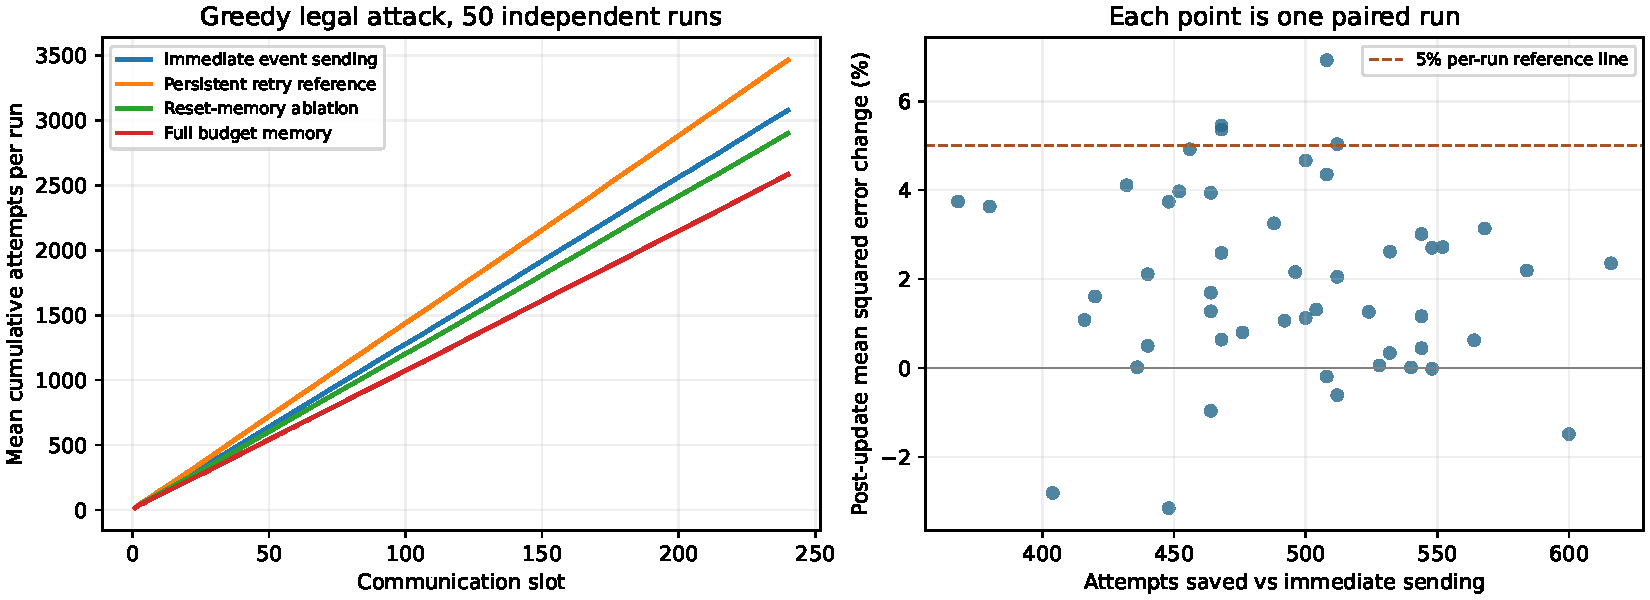
\includegraphics[width=.95\linewidth]{figures/greedy_results.pdf}
\caption{因果贪心攻击下的配对通信与误差结果。每个散点对应一组原始样本。\\ Figure~\thefigure\quad Paired communication and error results under causal greedy attacks}
\label{fig:greedy}
\end{figure}
\begin{figure}[htbp]
\centering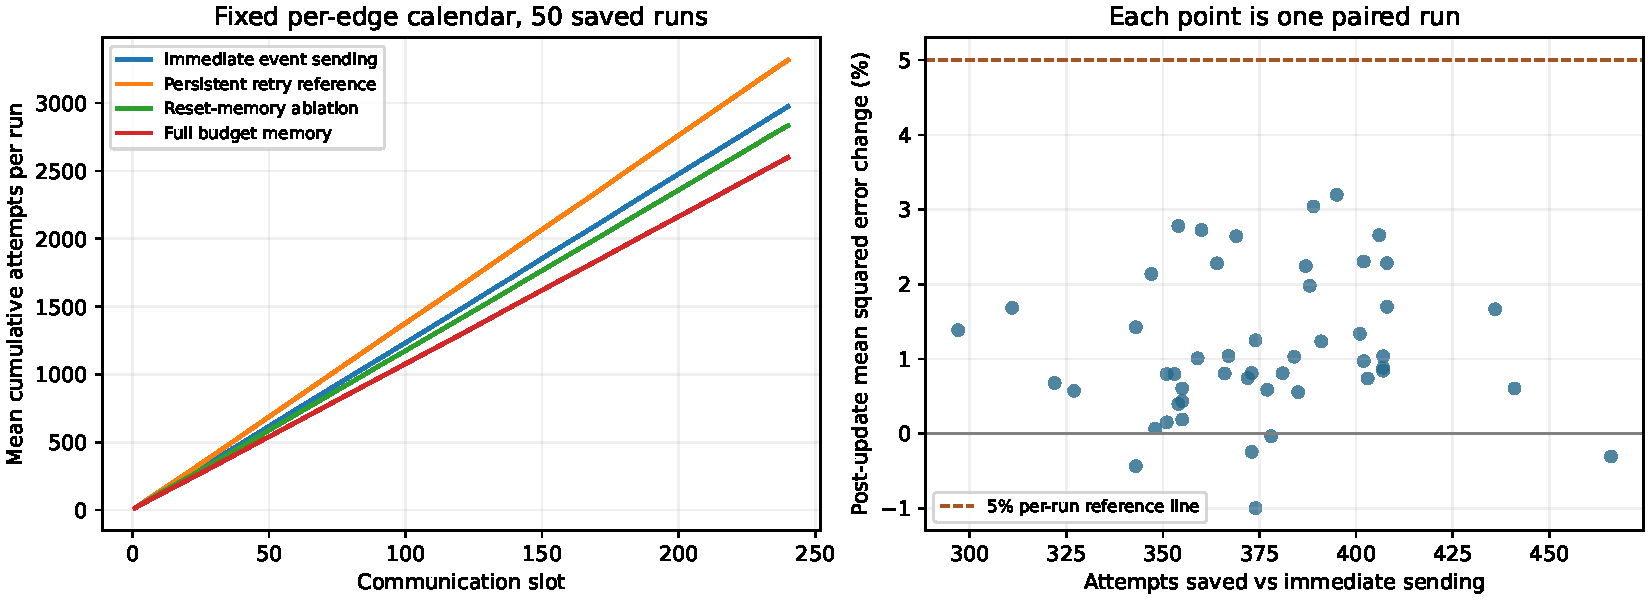
\includegraphics[width=.95\linewidth]{figures/calendar_results.pdf}
\caption{逐边异相日历下的配对结果，复用图\ref{fig:greedy}的50组原始样本。\\ Figure~\thefigure\quad Paired results under the heterogeneous link calendar using the same samples}
\label{fig:calendar}
\end{figure}

相对立即发送，每组平均净省包在贪心攻击下为493.04次，近似95\%配对$t$区间为$[477.54,508.54]$，单组范围为368--616次。异相日历下均值为375.32次，区间为$[366.22,384.42]$，单组范围为297--466次。相应平均误差差的近似区间分别为$[0.016490,0.033544]$和$[0.010837,0.019360]$。这些区间描述固定攻击规则下的样本不确定性。

误差代价也存在组间差异。相对立即发送，贪心攻击下43组误差增加、7组降低，4组增幅超过5\%，最大增幅约6.92\%。异相日历下45组增加、5组降低，最大增幅约3.20\%。5\%为探索阶段对全部样本、节点和时刻聚合平均误差变化的筛查值，不是每组或每节点的约束，应用精度验收需另给明确要求。无攻击时四协议逐拍结果相同，总尝试137632次，平均误差1.208413，实际延后数为零。

各节点的代价见表\ref{tab:node}。节点平均误差先对50组样本和240拍取平均。峰值定义为各时刻先对50组样本平均，再在240拍中取最大值，即
$\max_k\{50^{-1}\sum_m\|e_{i,k+1}^{(m)}\|^2\}$。
两类攻击下五个节点的平均误差均增加，贪心攻击下峰值的最大增幅约为4.32\%。该表给出有限样本误差曲线的统计量。
\begin{table}[htbp]
\centering\small
\caption{完整记忆相对立即发送的各节点误差增幅（\%）\\ Table~\thetable\quad Node error increases of full memory relative to immediate sending (\%)}\label{tab:node}
\begin{tabular}{lrrrr}
\toprule
Node & Greedy mean & Greedy peak & Calendar mean & Calendar peak\\
\midrule
1 & 2.171 & 3.215 & 1.177 & 1.102\\
2 & 1.486 & 4.318 & 1.341 & 1.642\\
3 & 2.156 & 3.100 & 1.171 & 1.518\\
4 & 1.468 & 3.862 & 1.205 & 2.063\\
5 & 2.185 & 3.476 & 1.109 & 1.078\\
\bottomrule
\end{tabular}
\end{table}


\subsection{独立校准固定阈值的比较}
为检查普通触发参数调整能否替代当前实验中的资源收益，另取主种子2026110901生成20组独立校准样本，每组240拍。完整记忆仍使用$\theta=0.2$。基准保持立即发送，阈值候选集在执行前固定为$\{0.20,0.21,\ldots,0.40\}$。每类攻击分别选择校准平均误差最接近完整记忆的阈值，之后锁定，在原50组测试样本上评价。贪心攻击选择$0.28$，异相日历选择$0.25$。这是按攻击条件分别离线校准的固定参数参考，不需要在线读取攻击状态，也不构成一个统一阈值的部署方案。

校准阶段，贪心下候选和所选基准的平均误差分别为1.335645、1.337834，日历下为1.278336、1.277368。测试集是已有样本的审稿追加比较，未用于本轮阈值选择。事前将测试聚合误差相差0.5\%以内作为描述性的接近标准，并报告全部结果。此标准不替代统计等效性检验或应用精度要求。

\begin{table}[htbp]\centering\small
\caption{独立校准后在原测试集上的结果\\ Table~\thetable\quad Test results after independent calibration}\label{tab:matched}
\begin{tabular}{llrrrrr}\toprule
Attack & Protocol & $\theta$ & Attempts & Failures & Successes & MSE\\\midrule
Greedy & Calibrated & 0.28 & 126084 & 73688 & 52396 & 1.347615\\
Greedy & Full memory & 0.20 & 129160 & 77944 & 51216 & 1.330751\\
Calendar & Calibrated & 0.25 & 128367 & 51045 & 77322 & 1.273858\\
Calendar & Full memory & 0.20 & 129982 & 59598 & 70384 & 1.277224\\
\bottomrule\end{tabular}
\end{table}

异相日历下，普通触发以128367次尝试得到平均误差1.273858，完整记忆为129982次和1.277224。候选比校准基准多发1.258\%，误差高0.264\%，五个节点的聚合误差也均较高。因而该测试条件没有提供预算记忆更优的经验资源折中证据。贪心下，候选比校准基准多发2.440\%，但误差低1.251\%，误差偏差超过事前0.5\%标准，应解释为两个不同的折中点。

\begin{table}[htbp]\centering\small
\caption{校准比较中的逐节点平均误差\\ Table~\thetable\quad Mean error by node in the calibrated comparison}
\begin{tabular}{llrrrrr}\toprule Attack & Protocol & Node 1 & Node 2 & Node 3 & Node 4 & Node 5\\\midrule
Greedy & Calibrated & 1.421673 & 1.233401 & 1.424153 & 1.234483 & 1.424368\\
Greedy & Full memory & 1.405547 & 1.215934 & 1.408357 & 1.215636 & 1.408279\\
Calendar & Calibrated & 1.348713 & 1.156727 & 1.353043 & 1.157747 & 1.353060\\
Calendar & Full memory & 1.350091 & 1.163502 & 1.354950 & 1.163202 & 1.354376\\
\bottomrule\end{tabular}
\end{table}

以独立运行作为统计单位，候选相对校准基准的每组净省包均值，贪心下为$-61.52$次，近似95\%配对$t$区间为$[-80.52,-42.52]$，仅9/50组省包。日历下为$-32.30$次，区间为$[-43.61,-20.99]$，13/50组省包。候选减基准的平均误差差及其区间，分别为$-0.016865$、$[-0.029229,-0.004501]$，以及$0.003366$、$[0.000053,0.006679]$。逐组最大相对误差退化分别为5.581\%和2.466\%，超过5\%的组数为1和0。这些统计量条件于已选择阈值，不涵盖重新选择校准样本的变异，也不是全攻击类结论。

阈值改变后，比较矩阵$M$保持不变，式\eqref{eq:comparison}中的阈值输入随之改变。重新用有理数计算相应全时刻包络，并检查初值包含，结果见表\ref{tab:matchedcert}。调大阈值使该理论上界变大，不能将新基准归入原$\theta=0.2$的同一数值证书。
\begin{table}[htbp]\centering\small
\caption{各阈值下重新计算的节点均方上界\\ Table~\thetable\quad Recomputed node mean-square bounds}\label{tab:matchedcert}
\begin{tabular}{lrrr}\toprule Threshold & Nodes 1,3,5 & Nodes 2,4 & Node average\\\midrule
0.2 & 3391.677 & 1783.994 & 2748.604\\
0.25 & 3477.131 & 1827.269 & 2817.186\\
0.28 & 3528.914 & 1853.483 & 2858.742\\
\bottomrule\end{tabular}
\end{table}

这一对照没有推翻固定截止安全等待定理，也没有证明预算记忆在所有场景均无资源价值。但当前证据未通过相近实际误差下的通信优势检验。本文因此仅主张精确安全动作边界、相应网络有界性及限定基准的数值行为，不主张通信成本最优或普通阈值调整无法替代的精度资源优势。

\subsection{后续发送、异质缓存与实现核验}
贪心攻击下，完整记忆共出现30240次延后，其中8140次随后低偏差取消、21980次随后实际发送、120次到时域末仍未决。异相日历下分别为22847、6237、16521和89次。当前参数由式\eqref{eq:cycle}保证一个锚点周期至多延后一拍，因而这些延后事件可以逐一追踪。取消数量反映一种节约机会，最终净成本仍由各闭环的总尝试数之差计算。

在$k=5,20,60,120,240$，相对立即发送的每组平均累计省包，贪心攻击下依次为9.68、34.24、122.16、241.60、493.04，异相日历下为5.74、28.30、92.12、186.38、375.32。在已固定的240拍时域内，后续发送保留了正向总收益。

异相日历的60000个“运行、发送节点、时刻”单元中，59883个单元的四条出边缓存至少一处相差超过$10^{-9}$，45486个单元存在出边发送动作差异。结果覆盖了各边独立缓存和不同ACK历史的实际运行。

实现核验独立于仿真主更新函数，从保存数组重放触发、占用计数、滑窗预算、成功载荷、同步缓存、锚点及式\eqref{eq:yang}。既有两批验证共600套闭环、2880000个边时刻，最大锚点年龄均为2，网络更新最大数值残差约$1.14\times10^{-13}$。有限整数枚举另覆盖36组$B,L$及25344个等待情形，检查式\eqref{eq:extension}的中间窗口。新增100套校准基准测试闭环也从日志独立重放，并重新核对已有200套候选及普通基准闭环，目标均为$x_2,\ldots,x_{241}$。一般参数的保证由理论证明给出。

按第\ref{sec:online}节队列删除顺序，对完整记忆在三类攻击条件下的720000次边决策进行复算，得到与完整失败日志相同的占用计数及发送动作。当前预算下队列最多保存2条失败时间戳，验证了有限窗口信息足以执行该规则。

\section{结论}
本文将可信ACK确认的历史阻断按未来锚点截止窗口重新计数，得到有限DoS预算下的安全发送延后规则。固定截止要求下的最大可保证等待长度具有闭式表达，跨成功保留的每条有效失败记录增加一个可认证等待时隙。所提规则保持有限锚点年龄，并在所用对角系统和固定增益条件下与立即发送共享均方误差证书。

独立保留样本和异相链路检查显示，在两类指定攻击下，完整记忆相对立即发送获得约12.62\%--16.03\%的总尝试节约，同时伴随约1.20\%--1.92\%的平均平方误差增加。追加的独立校准基准比较没有支持更优的经验资源折中。异相日历下，普通触发在略低误差下还减少了尝试，贪心下误差匹配未达到预定接近标准。共同理论证书认证均方有界，不能将同阈值下的省包直接扩展为同实际精度优势。普遍通信成本排序、无限时域节约率以及更紧的应用精度认证仍有待研究。指定近邻核对为当前机制差异提供了依据，贡献定位集中于截止窗口占用的精确安全等待边界及其分布式估计接口。

\begin{center}
\textbf{ACK-Based Safe Transmission Deferral under a Finite Attack Budget}
\end{center}
\noindent\textbf{Abstract}\quad This study addresses the communication cost of event-triggered distributed state estimation under denial-of-service (DoS) attacks with a hard sliding-window budget. A safe transmission-deferral mechanism is developed using trusted acknowledgement (ACK) feedback. Each directed link retains confirmed blocking timestamps and counts the records that remain valid in a future anchor-deadline window. An anchor is established by either a successful reception or a residual at or below the triggering threshold. The resulting budget occupancy determines whether an above-threshold request can wait. For a fixed deadline, a feasible history, and at most one attempt per slot, the maximum guaranteed initial waiting time is characterized exactly. Necessity follows from a legal blocking continuation across all overlapping windows. Independent, nondegenerate Gaussian measurement noise establishes positive-probability deadline failure when an inadmissible deferral is taken in the physical network. Retaining valid blocking records across successful receptions enlarges the certified waiting space by an explicit amount. The online rule preserves a bounded anchor age and a common mean-square error certificate for the fixed Yang-type estimator with per-link caches. Evaluation uses fifty independent held-out Gaussian noise samples, each spanning 240 communication slots. Each protocol evolves its estimates, caches, triggering decisions, and attack interactions independently on the same paired physical inputs. Under causal greedy attacks, total attempts decrease by 16.03 percent relative to immediate event sending, while the sample-averaged squared error increases by 1.92 percent. A fixed heterogeneous link calendar gives a 12.62 percent attempt reduction and a 1.20 percent error increase. Memory ablation and a persistent-retry reference support the mechanism assessment. A further baseline threshold is selected using twenty independent calibration samples for each attack condition. On the existing test samples, the calendar-calibrated immediate sender uses fewer attempts and has a slightly lower empirical error than the proposed mechanism. The greedy comparison does not meet the predefined error-closeness screen. Thus the results support the fixed-deadline safety characterization and mean-square boundedness, but do not establish a superior empirical communication--accuracy trade-off.

\noindent\textbf{Key words}\quad distributed state estimation; event-triggered communication; denial-of-service attacks; sliding-window budget; acknowledgement memory

\newcommand{\doi}[1]{\href{https://doi.org/#1}{\nolinkurl{#1}}}
\begin{thebibliography}{9}
\bibitem{Paper_Yang2014_StochasticActivation}
YANG W, CHEN G, WANG X, et al. Stochastic sensor activation for distributed state estimation over a sensor network[J]. Automatica, 2014, 50, 2070--2076. \doi{10.1016/j.automatica.2014.05.025}.

\bibitem{Paper_FUS33_2022}
SUN Y C, YANG G H. Event-Triggered Distributed State Estimation for Multiagent Systems Under DoS Attacks[J]. IEEE Transactions on Cybernetics, 2022, 52(7), 6901--6910. \doi{10.1109/TCYB.2020.3034456}.

\bibitem{Paper_FUS42_2022}
LEI H, YANG W, YU Y. Energy efficient management for distributed state estimation under DoS attacks[J]. International Journal of Robust and Nonlinear Control, 2022, 32(4), 1941--1959. \doi{10.1002/rnc.5898}.

\bibitem{Paper_FUS37_2023}
BASIT A, TUFAIL M, REHAN M, et al. Distributed State and Unknown Input Estimation Under Denial-of-Service Attacks: A Dynamic Event-Triggered Approach[J]. IEEE Transactions on Circuits and Systems II: Express Briefs, 2023, 70(6), 2266--2270. \doi{10.1109/TCSII.2022.3229412}.

\bibitem{Paper_FUS06_Sun2024}
SUN H T, PENG C, SHEN Y. Attack-Detection-Based Event-Triggered Transmission Scheme for Stabilizing Cyber-Physical Systems Under Denial of Service Attacks[J]. IEEE Transactions on Industrial Cyber-Physical Systems, 2024, 2, 176--184. \doi{10.1109/TICPS.2024.3419057}.

\bibitem{Paper_FUS47_2017}
DOLK V, HEEMELS M. Event-triggered control systems under packet losses[J]. Automatica, 2017, 80, 143--155. \doi{10.1016/j.automatica.2017.02.029}.

\bibitem{Paper_FUS48_Ding2016}
DING K, REN X, SHI L. Deception-based Sensor Scheduling for Remote Estimation under DoS Attacks[J]. IFAC-PapersOnLine, 2016, 49(22), 169--174. \doi{10.1016/j.ifacol.2016.10.391}.
\bibitem{Paper_FUS46_2020}
GUO L, YU H, HAO F. Event-triggered control for stochastic networked control systems against Denial-of-Service attacks[J]. Information Sciences, 2020, 527, 51--69. \doi{10.1016/j.ins.2020.03.045}.

\bibitem{Paper_FUS50_Zhao2024}
ZHAO M, QIN W, YANG J, et al. Security control for cyber-physical systems under aperiodic denial-of-service attacks: A memory-event-triggered active approach[J]. Neurocomputing, 2024, 600, 128159. \doi{10.1016/j.neucom.2024.128159}.
\end{thebibliography}


\clearpage
\section*{图文摘要}
\begin{center}
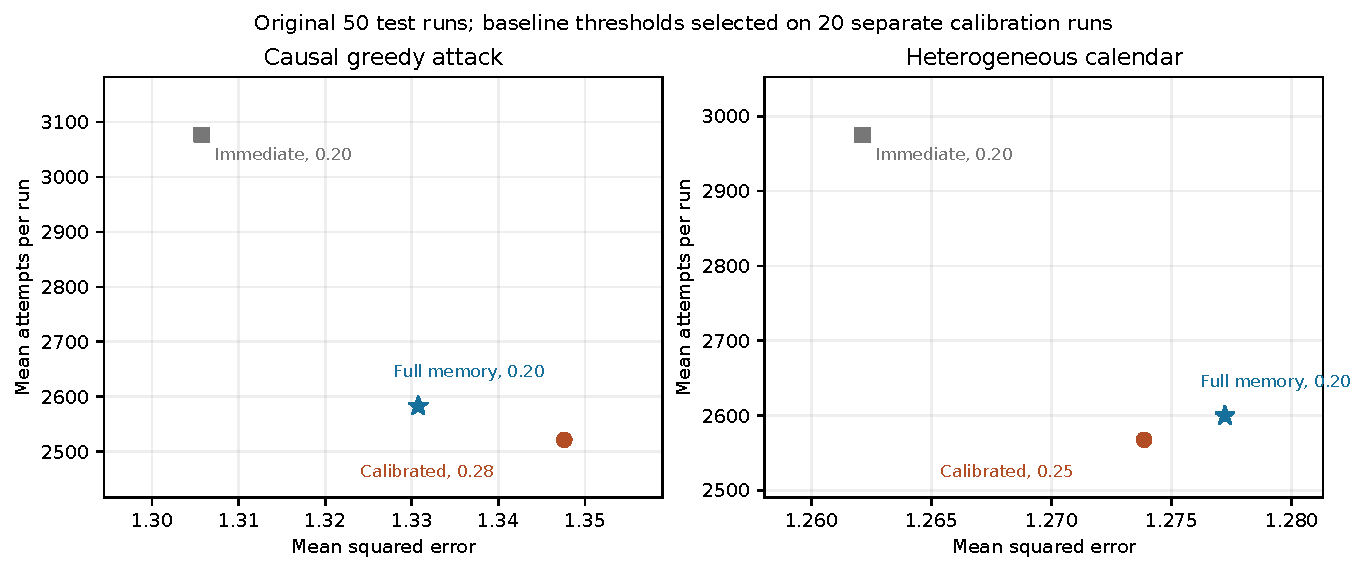
\includegraphics[width=\linewidth]{figures/matched_tradeoff.pdf}
\end{center}
\noindent
Confirmed blocking timestamps retained across successful transmissions enlarge safe waiting opportunities.
The rule preserves mean-square boundedness. A separately calibrated immediate-sending baseline
limits the empirical communication--accuracy advantage claimed for the mechanism.

\end{document}
